\documentclass{beamer}

\usetheme{default}
\usecolortheme{default}

\usepackage{graphicx} % Allows including images
\usepackage{booktabs} % Allows the use of \toprule, \midrule and \bottomrule in tables
\setbeamertemplate{caption}{\insertcaption} 
\setbeamertemplate{caption label separator}{}
\setbeamerfont{frametitle}{size=\Large}

\newenvironment{graytext}{\color{gray}}{\ignorespacesafterend}

\begin{document}

%------------------------------------------------
%------------------------------------------------

\section{Introduction}

%------------------------------------------------
%------------------------------------------------

\begin{frame}

\frametitle{Tasks}

\textbf{Cognition:} 3DMR, Corsi, Perspective-taking \\
\vspace{0.75cm}
\textbf{Anxiety:} Harm-avoidance, Spatial anxiety \\
\vspace{0.75cm}
\textbf{Navigation:} Pointing task \\
\vspace{0.75cm}
\textbf{Mobility:} Trackers (daily), Interviews (annual, lifetime)

\end{frame}

%-------------------------------------------------

\begin{frame}

\frametitle{Sex Differences}
\begin{table}
\begin{tabular}{l c c c}
\toprule
\textbf{Measure} & \textbf{N (m:f)} & \textbf{Std. $\beta$} & \textbf{p-value}\\ 
\midrule
3DMR & 52:54 & .20 & \emph{.037}\\
Corsi & 57:48 & .26 & \emph{.007}\\
Perspective-taking & 56:44 & -.31 & \emph{.002}\\
Harm avoidance & 27:27 & -.19 & .177\\
Spatial Anxiety & 26:27 & -.35 & \emph{.009}\\
Pointing & 61:57 & -.21 & \emph{.023}\\
Daily mobility & 20:18 & .45 & \emph{.004}\\
Annual mobility & 42:45 & .34 & \emph{.001}\\
Lifetime mobility & 58:60 & .39 & \emph{.000}\\
\bottomrule
\end{tabular}
\end{table}

\end{frame}

%------------------------------------------------

\begin{frame}
\frametitle{Perspective-taking}
\begin{figure}
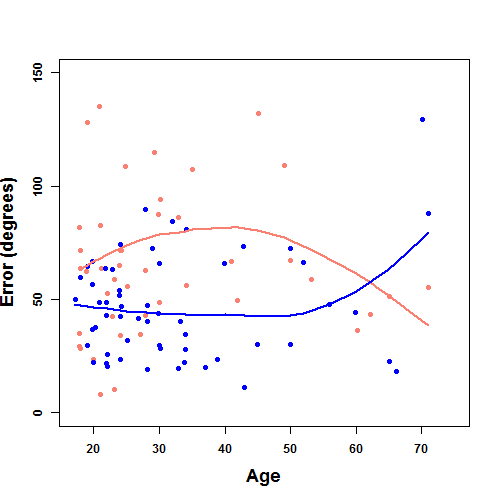
\includegraphics[width=0.75\linewidth]{prspage}
\end{figure}
\end{frame}

%-------------------------------------------------

\begin{frame}
\frametitle{Daily mobility}
\begin{figure}
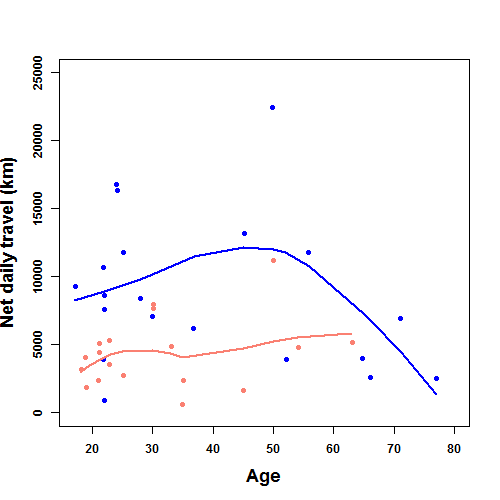
\includegraphics[width=0.75\linewidth]{tracking}
\end{figure}
\end{frame}

%-------------------------------------------------

\begin{frame}

\frametitle{Inter-task correlations}

\begin{table}
\begin{tabular}{l c c c}
\toprule
\textbf{Cognition} & 3DMR & Corsi & Persp.\\ 
\midrule
3DMR & - & -.08 & .07\\
Corsi & -.08 & - & \textbf{.25*}\\
Persp. & .07 & \textbf{.25*} & - \\
\bottomrule
\end{tabular}
\end{table}

\begin{table}
\begin{tabular}{l c c c}
\toprule
\textbf{Mobility} & Daily & Annual & Life\\ 
\midrule
Daily & - & .13 & \textbf{.20*}\\
Annual & .13 & - & \textbf{.32*}\\
Life & \textbf{.20*} & \textbf{.32*} & - \\
\bottomrule
\end{tabular}
\end{table}

\end{frame}

%------------------------------------------------

\begin{frame}
\frametitle{Cognition and survey knowledge}
\begin{figure}
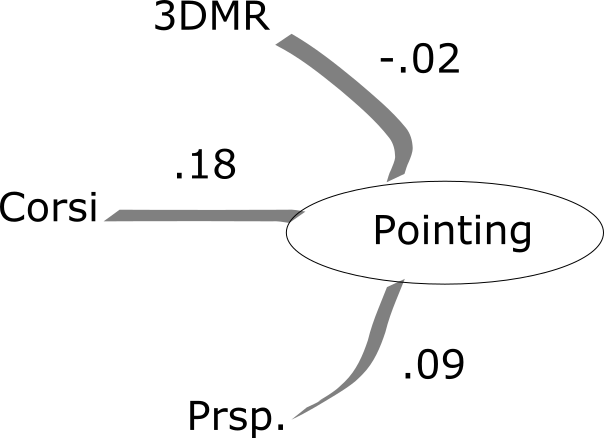
\includegraphics[width=0.65\linewidth]{cognav}
\end{figure}
\end{frame}

%-------------------------------------------------

\begin{frame}

\frametitle{Other relationships....}

\emph{Cognition and mobility}: Nothing\\
\vspace{0.75cm}
\emph{Navigation and mobility}: Nothing\\
\vspace{0.75cm}
\emph{Anxiety and cognition}: Only 17 participants... Nothing\\
\vspace{0.75cm}
\emph{Anxiety and mobility}: Only 17 participants... wonky results...\\

\end{frame}

%-------------------------------------------------

%\begin{frame}
%\frametitle{Huh??...}

%\begin{table}[h]
%\caption {\textbf{Harm avoidance and mobility}}
 % \centering
  %\begin{tabular}{| l | l l l|} 
 % 	\hline
%	& HA & Male & $R^2$ \\ \hline
%	M1 & .54* & & .26 \\
%	M2 & .62** & .49* & .49 \\ \hline
%  \end{tabular}
%\end{table}
%\end{frame}

%------------------------------------------------

\begin{frame}

\frametitle{Human Nature}

\textbf{Women's mobility}: Looked at men previously. Time for the women \\
\vspace{0.75cm}
\textbf{Fertility and parental care}: Risk aversion.  Energy preservation. Both should peak during fertility and when with dependent children. \\
\vspace{0.75cm}
\textbf{Related issues}: Burden of childcare.  Great Apes and infanticide avoidance.\\

\end{frame}

%-------------------------------------------------

\begin{frame}

\frametitle{Hypotheses}

\textbf{H1}: Women are more risk averse than men. \\
\vspace{0.75cm}
\textbf{H2}: Women are less mobile than men. \\
\vspace{0.75cm}
\textbf{H3}: Women will have lowest mobility and highest anxiety during peak reproductive years. \\
\vspace{0.75cm}
\textbf{H4}: These patterns will be exaggerated among women with young dependents. \\

\end{frame}

%-------------------------------------------------

\begin{frame}
\frametitle{Women's mobility by age}
\begin{figure}
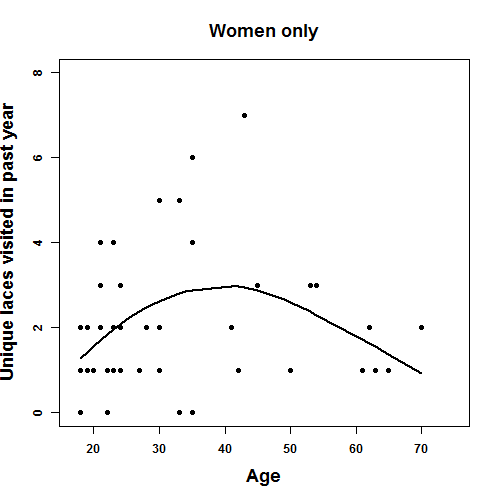
\includegraphics[width=0.65\linewidth]{justwom}
\end{figure}
\end{frame}

%-------------------------------------------------

\begin{frame}
\frametitle{Women vs. Men}
\begin{figure}
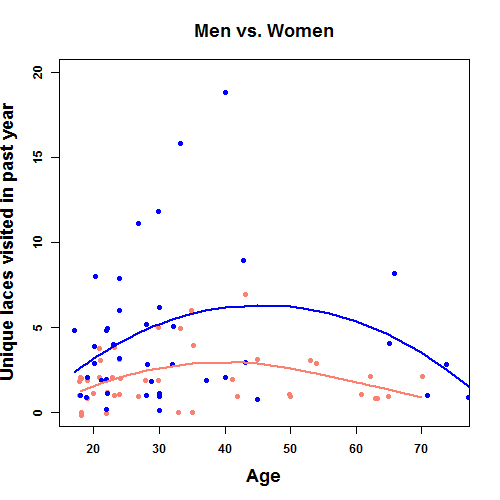
\includegraphics[width=0.65\linewidth]{menwom}
\end{figure}
\end{frame}

%-------------------------------------------------

\begin{frame}
\frametitle{Mobility of women with young dependents}
\begin{figure}
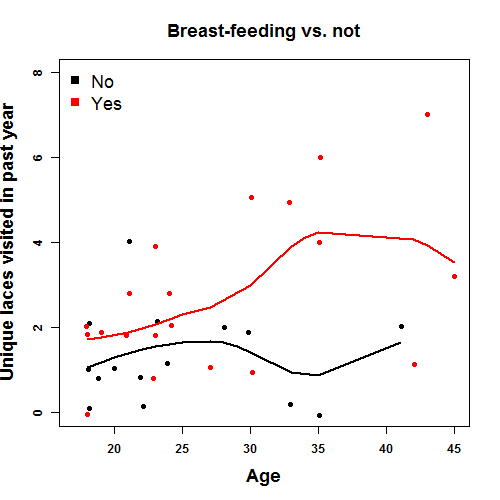
\includegraphics[width=0.65\linewidth]{bfeed_mob}
\end{figure}
\end{frame}

%-------------------------------------------------

%\begin{frame}
%\frametitle{Anxiety of women with young dependents}
%\begin{figure}
%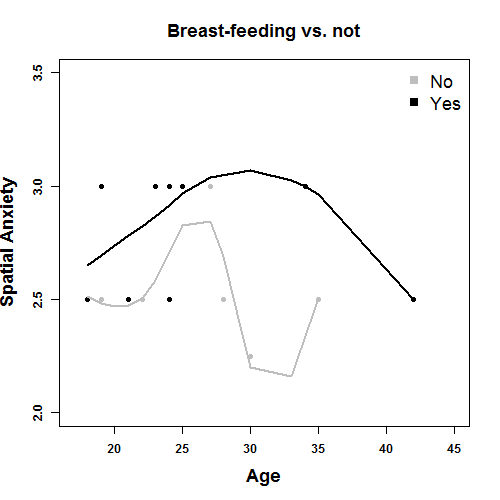
\includegraphics[width=0.65\linewidth]{bfeed_anx}
%\end{figure}
%\end{frame}

%-------------------------------------------------


\end{document}
